\chapter{Feature Extraction}\label{chap:feature}
A toxicology screening can be observed as a typical two-class classification problem, consisting of feature extraction and classification process. In this chapter we will explain feature extraction algorithm for ISV and CVP.

\section{Intersegmental Vessel Feature Extraction}
ISV features are defined in terms ISV count; an average distance between ISV, total area of ISV; and an average ISV length. All terms were defined in pixels. Previous research have shown the quantification terms used in this work can use to analyze toxicity effect in ISV \cite{Feng05}, \cite{Tran07}, \cite{Vogt09}.

\begin{figure}[H]
  \begin{center}
    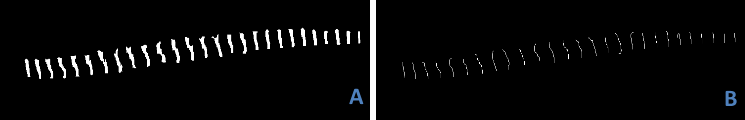
\includegraphics[scale=0.7]{figure/skeleton.png}
  \end{center}
  \caption[ISV skeleton]{Skeleton of ISV, used for calculating length of ISV.} 
  \label{skeleton}
\end{figure}

Our quantification procedure consists of reporting features: ISV count; average distance between ISV; total area of ISV; and average ISV length. We calculate these features for each of embryo. Features are obtained by performing connected component analysis. Number of connected component corresponds to ISV count. ISV distance is computed as the average of euclidean distance between ISV centroid, and the centroid of two adjacent neighboring ISV. Total area occupied by all components is ISV area. ISV length is computed by analyzing the skeleton of each of connected component. Image skeleton is obtained by thinning procedure explained in \cite{Lee94}.The general idea is to erode the ISVs surface iteratively until only the skeleton remains. The structure obtained is shown in fig. \ref{skeleton}(b). We decompose each individual vessel segments as individual graph for calculating ISV length. We perform graph analysis on each vessel and compute end points (pixels with less than 2 neighbors). For calculating the length of ISV we find the number of pixels connecting the end points. Average ISV length is computed by averaging over all graphs. Feature vector is formed by concatenating ISV count; average distance between ISV; total area of ISV; and average ISV length. 

\section{Caudal Vein Plexus Feature Extraction}\label{sec:cvp}
The study of the zebrafish CVP and its utilization as a model for screening assay has not been as prevalent as the ISV, and very few studies have attempted to identify regulators of CVP development. Previous research has primarily focused on using color, texture \cite{Tran07} and morphological changes \cite{Feng05} for toxicity analysis. Shape information, however, can be another attribute that can be evaluated. A shape descriptor can capture the outline of the shape that other color or texture-based descriptors may not be able to capture. Hence by quantification of the shape of CVP, and comparing it against that of a healthy embryo, we can identify changes in CVP due to exposure to toxins. This section will discuss utilization of gray level co-occurrence matrix (GLCM), histogram of oriented gradients (HOG), co-occurrence of histogram of oriented gradients gradient (Co-HOG) and weighted co-occurrence histogram of oriented gradients (gCo-HOG) for shape modeling.


\subsection{Gray Level Co-occurrence Matrix}

GLCM is a very well known texture analysis method \cite{haralick1973}, \cite{haralock1991}.  GLCM represents the angular and spatial over an image sub region. GLCM entries represents an estimate of the probability that two pixels with a specified displacement, d, and an angle, $\theta$ occurs in an image.  Statistical measures are derived from the co-occurrence matrix. The features we used include: energy, homogeneity, correlation, and contrast. For varying choices of d and $\theta$, we obtain a separate GLCM. The GLCM is implemented with certain degree of rotation invariance, which is achieved by combining the results from various angles. Angles 0, 45, 90, 135 are considered as effective choices. We analyzed results with varying value of k and obtained best performance with 9 pixel displacement. The results is combined by averaging the GLCM for each angle and concatenating energy, homogeneity, correlation, and contrast into one feature vector.

\subsection{Histogram of Oriented Gradients}

HOG descriptor first proposed by Dalal and Triggs \cite{Dalal05} has been used in many different problems in computer vision, such as pedestrian detection \cite{Wada09}, face recognition \cite{Deniz11}, object recognition \cite{Bosch07} and text recognition \cite{Wang10}. HOG features are extracted from image by first computing gradient orientation at every pixel. Orientations of gradients are quantized into histogram bins and each bin has an orientation range. Image is divided into blocks and in each block a histogram of oriented gradients is computed. HOG feature consists of concatenation of histogram of oriented gradients over all blocks. 

\begin{figure}[htb] 
 \centering
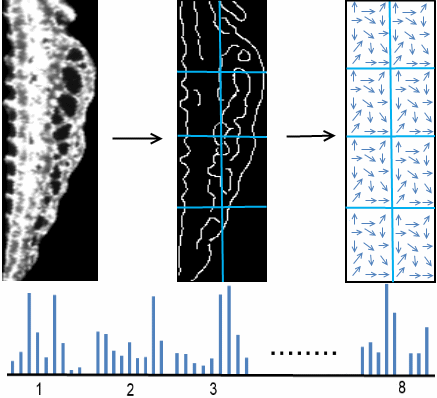
\includegraphics[scale=0.75]{figure/hog.png}
  \caption[HOG features from a CV image]{Extraction of HOG features from a CV image. (left) Original image. (center) Edge contours are extracted using an edge detector, image is divided into 8 blocks. (right) HOG vector is extracted from each sub region. (bottom) Concatenation of all the HOG vectors to obtain the HOG features for image.}
 \label{hog}
\end{figure}

In our case, HOG are computed on edge contours extracted using the canny edge detector (fig. \ref{hog}(center)). The gradients are computed using a Sobel mask. The HOG descriptor is quantized into $K$ orientation bins, each over an orientation range. The weight from each contour point depends on its gradient magnitude and is added to its orientation bin. Each bin in the histogram represents the sum of gradient magnitudes that have orientations within a certain angular range. 

HOG are invariant to 2d rotation and illumination variations. On the other hand, HOG captures orientation of only isolated pixels, ignoring spatial relationship among neighboring pixels. Co-HOG captures spatial information and is more powerful in describing local structure. With spatial structure, more shape information of object can be captured.

\subsection{Co-occurrence of Histogram of Oriented Gradients}\label{sssec:cohog}

Co-HOG is an extension of HOG. Co-HOG captures spatial information by measuring probability of oriented gradients between pairs of pixel. A pixel pair can be represented by an offset $(x, y)$, which captures the spatial relationship of the two points. As shown in fig. \ref{cohog}(left), we define 31 offsets including zero offset for a given point. The black pixel in the center is the pixel under consideration and the neighboring blue pixels are with different offsets. Each neighboring pixel in blue color forms an orientation pair with the center black pixel and accordingly votes to the co-occurrence matrix. For each pixel in the image of size $M \times N$, the orientations ranging between $[0, 360]$ are quantized into eight orientation bins. Co-occurrence matrix at a specific offset $(x, y)$ is defined as:
		
			\begin{equation}\label{eq:cohog}
				C_{x,y}(i, j) = \sum_{p}\sum_{q}\begin{cases} 1, & \mbox{if } I(p, q) = i, I(p + x, q + y) = j\\ 
				0, &  otherwise \end{cases} 
				\end{equation} 
				\normalsize 
				
The Co-HOG descriptor is formed by concatenation of components of the co-occurrence matrix of each offset including offset 0. Co-HOG obtains 31 co-occurrence matrices. There are $8 \times 8 = 64$ elements in the co-occurrence matrix (fig \ref{cohog}(right)). The co-occurrence matrix calculated with zero offset has only 8 values.

%There are $8 \times 8 = 64$ elements in the co-occurrence matrix (fig \ref{cohog}(right)). The co-occurrence matrix calculated with zero offset has only 8 values. 8 rectangular regions are tiled $M/4 \times N/2$ with no overlap. More tiles are made along the image width as CV occupies more region along width as compared to height. Finally, co-occurrence matrices from all the rectangular regions are concatenated into one vector. Thus the dimension of our feature is $(64 \times 30 + 8) \times 8 = 15424$. 
Co-HOG extracts both local and global shape information, with varying offset sizes. 

One potential limitation of co-occurrence histograms of oriented gradients is that both strong and weak gradients provide the same contribution in representing the spatial structure.  To address this limitation, we investigate the inclusion of gradient strength in the generation of the histogram.

\begin{figure}[htb] 
 \centering
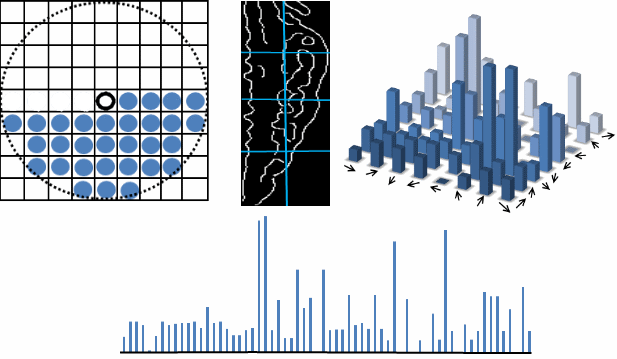
\includegraphics[scale=0.75]{figure/cohog.png}
  \caption[Co-HOG features from a CV image]{ Extraction of Co-HOG features from a CV image. (left) Pixel offset. (center) Edge contours are extracted using an edge detector, image is divided into 8 blocks. (right) Co-HOG vector is extracted from one region. (bottom) concatenation of all the Co-HOG vectors to obtain the Co-HOG features for image.}
 \label{cohog}
\end{figure}

As shown in \cite{Pang12}, we treat gradient as forces and use vector addition to combine forces using:
	
				\begin{equation}\label{eq:add}
				C_{x,y} = C_{x,y} + \|g_{1} + g_{2}\| 
				\end{equation}
				\normalsize 
				
where $C$ is the co-occurrence matrix at a specific offset $(x, y)$ as defined in equation \ref{eq:cohog}, $g_{1}$ is the gradient magnitude at location $(p, q)$, and $g_{2}$ is the gradient magnitude at location $(p + x, q + y)$. The gCo-HOG feature descriptor of the whole image can then be constructed by concatenating all the regions features. The gCo-HOG is normalized to sum to unity.

\section{Vasculature Time-lapse Features} \label{sec:timelapse}

There are various challenges associated with live imaging oz zebrafish. One such complication is, zebrafish embryos twitch, so that growth and motion of embryos are not uniform across the 3D field. Imaging captures the dynamics of blood vessel formation over time. In order to quantify these morphological changes, i.e. how much vascular structure has changed over a period of time, it is necessary to compensate for any movements caused by the growing embryo. Thus, in order to record the temporal changes occurring due to vessel growth, it is necessary to establish spatial correspondence between blood vessels that may appear displaced due to embryo movement. Thus quantification of temporal vascular growth can be seen as a problem of image registration. we use a non-rigid registration approach to align images. Non-rigid mapping is based on complete correspondence of images and includes a deformation model as the underlying transformation. We utilize free-form deformation based on B-splines for growth monitoring, and use intensity differences as a similarity measure.  

\subsection{Vasculature Registration}
The goal of image registration is to find an optimum mapping that aligns two images. Since deformations are important for quantification of changes in images, it is necessary to find a mapping between two time points as accurately as possible. In our case we need to quantify blood vessel growth independent of motion artifacts.  Hence we need a registration approach that establishes vessel correspondence between successive time frames. Affine and rigid registration approaches are mainly based on local stretching of images, and hence do not adequately capture structural changes.

Many applications in medicine require that object is modified in global scale. Therefore, we have used free-form deformation (FFD). Free form deformation deforms an object by warping the image geometry in which the object is localized. The nature of deformation varies widely across different time points; hence it is difficult to use traditional B-spline registration, which is based on many parameters. If we only select few parameters, an approximate match can be obtained, whereas many parameters incur added computational costs. Hence, we have used FFD based on hierarchical B-splines for multilevel nonlinear registration \cite{Lee97}. The underlying idea of FFD is based on deforming an object by manipulating a mesh of 2D points.

Let $\Omega  = \left\{(x,y)\mid 0 \leq\ x \geq X, 0 \leq\ y \geq Y \right\}$ be the domain of $2d$ points. Let $\Omega$ denote a $n_{x}\times n_{y}$ mesh of control points with uniform spacing $\Delta$. Let $\Omega_{ij}$ be the value of ij-th control point located at $(i,j)$. The FFD f can be written as:

\begin{equation}
f(x,y) = \sum_{m=0}^{3}\sum_{l=0}^{3}B_{l}(s)B_{m}(t)\Omega_{i+l,j+m}
\end{equation}	

where, 
$i = \floor*{\frac{x}{n_{x}}} - 1$ 
$j = \floor*{\frac{y}{n_{y}}} - 1$ ,
$s = \frac{x}{n_{x}} - \floor*{\frac{x}{n_{x}}}$,
$t = \frac{y}{n_{y}} - \floor*{\frac{y}{n_{y}}}$.
$B_{l}$ and $B_{m}$ are uniform cubic B-spline basis function defined as:

\begin{equation}
B_{0}(s)=  \frac{(1-s)^{3}}{6}
\end{equation}	
\begin{equation}
B_{1}(s)=  \frac{(3s^{3}-6s^{2}+4)^{3}}{6}
\end{equation}	
\begin{equation}
B_{2}(s)=  \frac{(-3s^{3}-3s^{2}+3s+1)^{3}}{6}
\end{equation}	
\begin{equation}
B_{3}(s)=  \frac{s^{3}}{6}
\end{equation}	

They weigh the contribution of each control point to $f(x,y)$ based on its distance to $(x,y)$. The problem of deriving function f is reduced to solving for the control points in $\Omega$. The control points in $\Omega$ behave as parameters for transformation. The degree of non-rigid deformation depends highly on the size of control points. Dense mesh can increase number of degrees of freedom, hence providing more flexibility and consequently an increase in computational complexity. In order to achieve the tradeoff between degree of freedom and computational complexity, we use a hierarchical multiresolution \cite{Lee97} approach, in which the resolution of the control mesh is increased, along with the resolution of image in an iterative loop. Consider a hierarchy of control mesh $\Omega_{0}, \Omega_{1},\ldots,\Omega_{h}$ overlaid on domain $\Omega$. For simplicity, we will assume decreasing space as we move from $\Omega_{s}$ to $\Omega_{s+1}$. Similar to above, we will have FFD $f_{s}(x,y)$ for each control mesh. Their sum defines the overall transformation model.

\begin{equation}
f(x,y)= \sum_{s=1}f_{s}(x,y)
\end{equation}
Calculation of FFD for each control lattice introduces a significant overhead. To avoid this overhead, B-spline refinement can be applied hierarchically to control mesh. This can be achieved by B-spline subdivision algorithm. In this case, the control point mesh at level s is generated by using the mesh control points from level $s-1$. More details can be found in \cite{Forsey88}. To achieve correspondence between two images acquired at different time points, we have used a similarity criterion based on sum of squared difference (SSD):

\begin{equation}
SSD = \frac{1}{n} \sqrt{(\sum{(I(t_{0})-T(I(t)))^{2}}}
\end{equation}

\subsection{Vasculature Morphology}\label{quantification}

Blood vessel growth is quantified by recording the temporal occurrence of differences in pixel intensities along registered vascular structures. Registration is performed on pair of consecutive images $(I_{t},I_{t+1})$. $I_{t}$ is warped to $I_{t+1}$ to give $I_{reg_t}$. Measuring the difference (pixel changed) between $I_{t+1}$ and $I_{reg_t}$  provides a standard for change quantification. This protocol is shown in fig. \ref{reg}

\begin{figure}[htb] 
 \begin{center}
    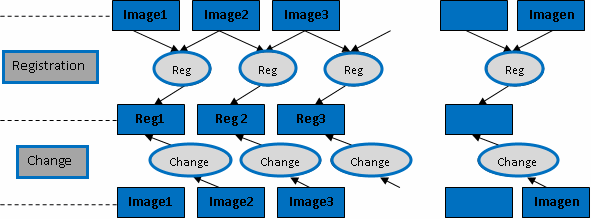
\includegraphics[scale=0.75]{figure/reg_overview.png}
  \end{center}
  \caption[Quantification Procedure]{For a given sequence of images, image i is registered to (i + 1). Measuring the difference between registered images i and (i + 1), provides the change in number of pixels.}
  \label{reg}
\end{figure}

, where $\Delta_{t}$  is the change in number of pixels at time t.
\begin{equation}
\Delta_{t}= I_{t+1} - I_{reg_t}
\end{equation} 


The change measured over the entire imaging cycle can be characterized by the function $f(\Delta_{t})$ given by:
\begin{equation}
f(\Delta_{t})= \left\{\delta_{t}\right\}_{t=1}^{m}
\end{equation}

In next chapter, we will give details corresponding to zebrafish data used for experiments.